\documentclass[11pt, english]{article}
%\usepackage[latin1]{inputenc}
\usepackage[T1]{fontenc}
\usepackage[utf8x]{inputenc}
\usepackage[english]{babel}   % S P R A A K
% \usepackage{graphicx}    % postscript graphics
\usepackage{amssymb, amsmath, amsthm, amssymb} % symboler, osv
\usepackage{mathrsfs}
\usepackage{url}
\usepackage{thmtools}
\usepackage{enumerate}  % lister $  
\usepackage{float}
\usepackage{tikz}
\usepackage{tikz-cd}
\usetikzlibrary{calc}
%\usepackage{tikz-3dplot}
\usepackage{subcaption}
\usepackage[all]{xy}   % for comm.diagram
\usepackage{wrapfig} % for float right
\usepackage{hyperref}
\usepackage{../mystyle} % stilfilen      
\usepackage{booktabs}
\usepackage{resizegather}
\setcounter{MaxMatrixCols}{48}
\usepackage{listings}
\lstset{language=Macaulay2}
\definecolor{mygreen}{rgb}{0,0.6,0}
\definecolor{mygray}{rgb}{0.5,0.5,0.5}
\definecolor{mymauve}{rgb}{0.58,0,0.82}

\lstset{ %
  backgroundcolor=\color{white},   % choose the background color; you must add \usepackage{color} or \usepackage{xcolor}
  basicstyle=\footnotesize,        % the size of the fonts that are used for the code
  breakatwhitespace=false,         % sets if automatic breaks should only happen at whitespace
  breaklines=true,                 % sets automatic line breaking
  captionpos=b,                    % sets the caption-position to bottom
  commentstyle=\color{mygreen},    % comment style
  deletekeywords={...},            % if you want to delete keywords from the given language
  escapeinside={\%*}{*)},          % if you want to add LaTeX within your code
  extendedchars=true,              % lets you use non-ASCII characters; for 8-bits encodings only, does not work with UTF-8
  frame=single,	                   % adds a frame around the code
  keepspaces=true,                 % keeps spaces in text, useful for keeping indentation of code (possibly needs columns=flexible)
  keywordstyle=\color{blue},       % keyword style
  language=Macaulay2,                 % the language of the code
  otherkeywords={*,...},           % if you want to add more keywords to the set
  numbers=left,                    % where to put the line-numbers; possible values are (none, left, right)
  numbersep=5pt,                   % how far the line-numbers are from the code
  numberstyle=\tiny\color{mygray}, % the style that is used for the line-numbers
  rulecolor=\color{black},         % if not set, the frame-color may be changed on line-breaks within not-black text (e.g. comments (green here))
  showspaces=false,                % show spaces everywhere adding particular underscores; it overrides 'showstringspaces'
  showstringspaces=false,          % underline spaces within strings only
  showtabs=false,                  % show tabs within strings adding particular underscores
  stepnumber=2,                    % the step between two line-numbers. If it's 1, each line will be numbered
  stringstyle=\color{mymauve},     % string literal style
  tabsize=2,	                   % sets default tabsize to 2 spaces
  title=\lstname                   % show the filename of files included with \lstinputlisting; also try caption instead of title
}

%\usepackage[a5paper,margin=0.5in]{geometry}

\begin{document}
\title{Calculations}
\author{Fredrik Meyer}
\maketitle

\tableofcontents 

\section{Computations on dP6}
\subsection{Finding equations of deformations}
%fra filen defcdp6.m2

Consider the del Pezzo surface $dP_6$ of degree 6 embedded in $\PP^6$. Its ideal is defined as follows:

\begin{lstlisting}
restart
S = QQ[x_1..x_6,y_0]
I = ideal(x_1*x_3-x_2*y_0,
    	x_2*x_4-x_3*y_0,
	x_3*x_5-x_4*y_0,
	x_4*x_6-x_5*y_0,
	x_5*x_1-x_6*y_0,
	x_6*x_2-x_1*y_0,
	x_1*x_4-y_0^2,
	x_2*x_5-y_0^2,
	x_3*x_6-y_0^2)
\end{lstlisting}

We compute the two deformations of its affine cone using the package \texttt{VersalDeformations}.

\begin{lstlisting}
(F,R,G,C) = versalDeformation(gens I);
decompose ideal transpose mingens ideal G
\end{lstlisting}

The output are four lists of matrices entries in $\Q[\mathbf x] \otimes \Q[t_1,t_2,t_3]$. The list $F$ consists of the equations of the family, and the list $R$ of the relations. The list $G$ gives equations for the base space. We have that $F_0$ is the matrix of generators of $I$, and that $F_i R_i \equiv 0 \pmod{t^{i+1}}$.

The decomposition of \texttt{ideal G} is the following:
\begin{lstlisting}
i9 : decompose ideal transpose mingens ideal G

o9 = {ideal(t  - t ), ideal (t  - t , t )}
             1    3           2    3   1

\end{lstlisting}

Thus the base space splits into two components meeting transversely at the origin, of dimension $2$ and $1$, respectively. By doing a change of variables we can get rid of the linear terms:

\begin{lstlisting}
T = QQ[x_1..x_6,y_0,t_1,t_2,t_3,s_1,s_2,s_3];
gsub = sub(sub(ideal mingens ideal G,T), {t_2 => s_2+s_3-s_1, t_1 => s_3, t_3 => s_3-s_1})
fsub = transpose  sub(sub(sum F,T), {t_2 => s_2+s_3-s_1, t_1 => s_3, t_3 => s_3-s_1})
\end{lstlisting}

Now the equations are easier:

\begin{lstlisting}
i13 : decompose gsub

o13 = {ideal(s ), ideal (s , s )}
              1           3   2

\end{lstlisting}

We can get equations for each of these families by setting $s_1=0$ and $s_3=s_2=0$, respectively:
\begin{lstlisting}
i25 : fsub1 = sub(fsub, s_1 => 0)

o25 = {-2} | x_1x_3-x_2y_0                            |
      {-2} | x_2x_4-x_3y_0+x_3s_2+x_3s_3              |
      {-2} | x_3x_5-x_4y_0+x_4s_3                     |
      {-2} | x_4x_6-x_5y_0                            |
      {-2} | x_1x_5-x_6y_0+x_6s_2+x_6s_3              |
      {-2} | x_2x_6-x_1y_0+x_1s_3                     |
      {-2} | x_1x_4-y_0^2+y_0s_2+y_0s_3               |
      {-2} | x_2x_5-y_0^2+y_0s_2+2y_0s_3-s_2s_3-s_3^2 |
      {-2} | x_3x_6-y_0^2+y_0s_3                      |

              9       1
o25 : Matrix T  <--- T
\end{lstlisting}

And:

\begin{lstlisting}
i26 : fsub2 = sub(fsub, {s_3 => 0, s_2 => 0})

o26 = {-2} | x_1x_3-x_2y_0        |
      {-2} | x_2x_4-x_3y_0-x_3s_1 |
      {-2} | x_3x_5-x_4y_0        |
      {-2} | x_4x_6-x_5y_0-x_5s_1 |
      {-2} | x_1x_5-x_6y_0        |
      {-2} | x_2x_6-x_1y_0-x_1s_1 |
      {-2} | x_1x_4-y_0^2-y_0s_1  |
      {-2} | x_2x_5-y_0^2-y_0s_1  |
      {-2} | x_3x_6-y_0^2-y_0s_1  |

              9       1
o26 : Matrix T  <--- T
\end{lstlisting}

\subsection{Intersecting with two special hyperplanes}
%fra filen defcdp6.m2

Consider $dP_6$ defined as above. Then consider the two hyperplanes
$$
h_1 = x_1+x_2+x_3+x_4+x_5+x_6
$$
and
$$
h_2 = x_1-x_2+x_3-x_4+x_5-x_6.
$$

We can compute the intersection with $dP_6$ in \texttt{Macaulay2} as follows:
\begin{lstlisting}
h1 = x_1+x_2+x_3+x_4+x_5+x_6
h2 = x_1-x_2+x_3-x_4+x_5-x_6

SS = S[r]/(r^2+3)
apply(decompose(sub(I + h1 + h2,SS)), j -> ideal mingens sub(j,y_0 => 1))
\end{lstlisting}

The reason we create a new ring is that we need $\sqrt{-3}$ in order for the ideals to decompose. The results is the following list of ideals:

\begin{enumerate}
	\item $(x_5-1,x_4+x_6+1,x_3+x_6+1,x_2-1,x_1-x_6,r-2x_6-1)$.
	\item $(x_5-1,x_4+x_6+1,x_3+x_6+1,x_2-1,x_1-x_6,r+2x_6+1)$.
	\item $(x_6-1,x_4-x_5,x_3-1,x_2+x_5+1,x_1+x_5+1,r-2x_5-1)$.
	\item $(x_6-1,x_4-x_5,x_3-1,x_2+x_5+1,x_1+x_5+1,r+2x_5+1)$.
	\item $(x_5-x_6,x_4-1,x_3+x_6+1,x_2+x_6+1,x_1-1,r-2x_6-1)$.
	\item $(x_5-x_6,x_4-1,x_3+x_6+1,x_2+x_6+1,x_1-1,r+2x_6+1)$.
\end{enumerate}


From this we can read off the coordinates in $\PP^6$:

\begin{table}[h]
\centering
\caption{Table of singular points.}
\label{singpoints}
\begin{tabular}{@{}lllllll@{}}
\toprule
$x_1$ & $x_2$ & $x_3$ & $x_4$ & $x_5$ & $x_6$ & $y_0$ \\ \midrule
$\frac{-1+\sqrt{3}}{2}$ & $1$ & $\frac{-1-\sqrt{-3}}{2}$ & $\frac{-1-\sqrt{-3}}{2}$ & $1$& $\frac{-1 + \sqrt{-3}}{2}$  & $1$ \\
 $\frac{-1+\sqrt{-3}}{2}$& 1 & $\frac{-1+\sqrt{-3}}{2}$ & $\frac{-1+\sqrt{-3}}{2}$ & 1& $\frac{-1-\sqrt{-3}}{2}$ & 1 \\
 $\frac{-1-\sqrt{-3}}{2}$ & $\frac{-1-\sqrt{-3}}{2}$ & 1  & $\frac{-1+\sqrt{-3}}{2}$  & $\frac{-1+\sqrt{-3}}{2}$ & 1& 1 \\
$ \frac{-1+\sqrt{-3}}{2}$ & $\frac{-1+\sqrt{-3}}{2}$ & 1  & $\frac{-1-\sqrt{-3}}{2}$ & $\frac{-1-\sqrt{-3}}{2}$ & 1& 1 \\
1& $\frac{-1-\sqrt{-3}}{2}$ & $\frac{-1-\sqrt{-3}}{2}$ & 1 & $\frac{-1+\sqrt{-3}}{2}$ & $\frac{-1+\sqrt{-3}}{2}$ & 1 \\
1& $\frac{-1+\sqrt{-3}}{2}$ & $\frac{-1+\sqrt{-3}}{2}$ & 1 & $\frac{-1-\sqrt{-3}}{2}$ & $\frac{-1-\sqrt{-3}}{2}$  & 1 \\ \bottomrule
\end{tabular}
\end{table}

Note that the hexagonal group $D_6$ act transitively on the set of singular points.

\subsection{Intersecting with another set of hyperplanes}
\label{sec:delpezzoz2}

Note that the group $\Z_2 \X \Z_2$ act on $dP_6$ by reflecting the triangulation in \figref{trianghexagon} (in fact $\Z_2 \x \Z_2$ is a subgroup of $D_6$). $\Z_2 \X \Z_2$ is the full symmetry group of the triangulation in the figure.


\section{Toric mirrors}

\subsection{First example}
\label{sec:toric5}

There are two examples of torics we have studied. The first one is this.

Let $I$ and $I'$ be the ideals of $dP_6$ with a disjoint set of variables. Let $J=I+I'$.

\begin{remark}
This is a deformation of the Stanley-Reisner scheme corresponding to the join of two hexagons and two points.
\end{remark}

Then $Y_0 = \Proj(S/J)$ is a toric variety whose associated polytope $P$ has vertices the column of the following matrix:

\begin{equation}
\left(
\begin{array}{rrrrrrrrrrrr}
0 & 0 & 0 & 0 & 0 & 0 & -2 & 2 & 0 & -2 & 0 & 2 \\
0 & 0 & 0 & 0 & 0 & 0 & 0 & 0 & -2 & -2 & 2 & 2 \\
-2 & 2 & 0 & -2 & 0 & 2 & 0 & 0 & 0 & 0 & 0 & 0 \\
0 & 0 & -2 & -2 & 2 & 2 & 0 & 0 & 0 & 0 & 0 & 0 \\
-1 & -1 & -1 & -1 & -1 & -1 & 1 & 1 & 1 & 1 & 1 & 1
\end{array}
\right)
\end{equation}

The polytope $P$ is reflexive with $87$ lattice points. We can use the Batyrev-Borisov construction to find a toric mirror candidate to $Y_0$.

The construction actually give two such families. Here's how: start with a reflexive polytope $P \subset M_\R$. A \emph{nef partition} induces a decomposition $V_1,V_2$ of the vertex set of $P^\vee \subset N_\R$, such that $P^\vee = \conv(V_1,V_2)$. Let $Q_i = \conv(V_i)$. Then one forms $Q := Q_1+Q_2 \subset N_\R$. Similarly, we have a dual nef partition, so that we can write $P = P_1 + P_2$.

A nef partition correspond to a complete intersection in $X_P$, and the dual nef partition correspond to a complete intersection in $X_Q$. 

We can find (using SAGE for example) the polytopes $P_1$ and $P_2$. They are given as follows:

\begin{equation}
P_1 = \conv
\left(\begin{array}{rrrrrrrrrrrr}
0 & 0 & 0 & 0 & 0 & 0 & 0 & 1 & 1 & 0 & -1 & -1 \\
0 & 0 & 0 & 0 & 0 & 0 & -1 & 0 & 1 & 1 & 0 & -1 \\
-1 & -1 & 1 & 0 & 1 & 0 & 0 & 0 & 0 & 0 & 0 & 0 \\
-1 & 0 & 1 & 1 & 0 & -1 & 0 & 0 & 0 & 0 & 0 & 0 \\
0 & 0 & 0 & 0 & 0 & 0 & 1 & 1 & 1 & 1 & 1 & 1
\end{array}\right)
\end{equation}
and
\begin{equation}
P_2 = \conv \left(\begin{array}{rrrrrrrrrrrr}
0 & 0 & 0 & 0 & 0 & 0 & 0 & 1 & 1 & 0 & -1 & -1 \\
0 & 0 & 0 & 0 & 0 & 0 & -1 & 0 & 1 & 1 & 0 & -1 \\
-1 & -1 & 1 & 0 & 1 & 0 & 0 & 0 & 0 & 0 & 0 & 0 \\
-1 & 0 & 1 & 1 & 0 & -1 & 0 & 0 & 0 & 0 & 0 & 0 \\
-1 & -1 & -1 & -1 & -1 & -1 & 0 & 0 & 0 & 0 & 0 & 0
\end{array}\right)
\end{equation}

There is a formula for the $Q_i$ given the $P_i$:
$$
Q_i = \{ u \in N_\R \mid \langle u,m \rangle \geq -1 \text{ for all } m \in P_i, \langle u,m\rangle \geq 0 \, \forall \, m \in P_j, j\neq i \}
$$

Then we find that $Q_1$ is given by
\begin{equation}
Q_1 = \conv \left(\begin{array}{rrrrrrr}
0 & 0 & 0 & 0 & 0 & 0 & 0 \\
0 & 0 & 0 & 0 & 0 & 0 & 0 \\
-1 & -1 & 0 & 0 & 0 & 1 & 1 \\
0 & 1 & -1 & 0 & 1 & -1 & 0 \\
-1 & -1 & -1 & 0 & -1 & -1 & -1
\end{array}\right)
\end{equation}
and
\begin{equation}
Q_2 = \conv \left(\begin{array}{rrrrrrr}
-1 & -1 & 0 & 0 & 0 & 1 & 1 \\
0 & 1 & -1 & 0 & 1 & -1 & 0 \\
0 & 0 & 0 & 0 & 0 & 0 & 0 \\
0 & 0 & 0 & 0 & 0 & 0 & 0 \\
1 & 1 & 1 & 0 & 1 & 1 & 1
\end{array}\right)
\end{equation}


The polytope $Q$ has $48$ vertices:
\begin{gather*}
  \setlength{\arraycolsep}{.5\arraycolsep}
  \text{\footnotesize$\displaystyle
\begin{pmatrix}
-1 & -1 & -1 & -1 & -1 & -1 & -1 & -1 & -1 & -1 & -1 & -1 & -1 & -1 & 0 & 0 & 0 & 0 & 0 & 0 & 0 & 0 & 0 & 0 & 1 & 0 & 0 & 0 & 0 & 0 & 0 & 0 & 0 & 0 & 0 & 1 & 1 & 1 & 1 & 1 & 1 & 1 & 1 & 1 & 1 & 1 & 1 & 1 \\
0 & 0 & 0 & 0 & 0 & 0 & 0 & 1 & 1 & 1 & 1 & 1 & 1 & 1 & -1 & -1 & -1 & -1 & -1 & -1 & -1 & 0 & 0 & 0 & 0 & 0 & 0 & 0 & 1 & 1 & 1 & 1 & 1 & 1 & 1 & -1 & -1 & -1 & -1 & -1 & -1 & -1 & 0 & 0 & 0 & 0 & 0 & 0 \\
-1 & -1 & 0 & 0 & 0 & 1 & 1 & -1 & -1 & 0 & 0 & 0 & 1 & 1 & -1 & -1 & 0 & 0 & 0 & 1 & 1 & -1 & -1 & 0 & 1 & 0 & 1 & 1 & -1 & -1 & 0 & 0 & 0 & 1 & 1 & -1 & -1 & 0 & 0 & 0 & 1 & 1 & -1 & -1 & 0 & 0 & 0 & 1 \\
0 & 1 & -1 & 0 & 1 & -1 & 0 & 0 & 1 & -1 & 0 & 1 & -1 & 0 & 0 & 1 & -1 & 0 & 1 & -1 & 0 & 0 & 1 & -1 & 0 & 1 & -1 & 0 & 0 & 1 & -1 & 0 & 1 & -1 & 0 & 0 & 1 & -1 & 0 & 1 & -1 & 0 & 0 & 1 & -1 & 0 & 1 & -1 \\
0 & 0 & 0 & 1 & 0 & 0 & 0 & 0 & 0 & 0 & 1 & 0 & 0 & 0 & 0 & 0 & 0 & 1 & 0 & 0 & 0 & -1 & -1 & -1 & 0 & -1 & -1 & -1 & 0 & 0 & 0 & 1 & 0 & 0 & 0 & 0 & 0 & 0 & 1 & 0 & 0 & 0 & 0 & 0 & 0 & 1 & 0 & 0
\end{pmatrix}
  $}
\end{gather*}

The polar polytope $Q^\vee$ is given by

\begin{gather*}
  \setlength{\arraycolsep}{.5\arraycolsep}
  \text{\footnotesize$\displaystyle
\begin{pmatrix}
-1 & -1 & -1 & -1 & 0 & 0 & 0 & 0 & 0 & 0 & 0 & 0 & 0 & 0 & 0 & 0 & 0 & 0 & 0 & 0 & 1 & 1 & 1 & 1 \\
-1 & -1 & 0 & 0 & -1 & -1 & 0 & 0 & 0 & 0 & 0 & 0 & 0 & 0 & 0 & 0 & 0 & 0 & 1 & 1 & 0 & 0 & 1 & 1 \\
0 & 0 & 0 & 0 & 0 & 0 & -1 & -1 & -1 & -1 & 0 & 0 & 0 & 0 & 1 & 1 & 1 & 1 & 0 & 0 & 0 & 0 & 0 & 0 \\
0 & 0 & 0 & 0 & 0 & 0 & -1 & -1 & 0 & 0 & -1 & -1 & 1 & 1 & 0 & 0 & 1 & 1 & 0 & 0 & 0 & 0 & 0 & 0 \\
0 & 1 & 0 & 1 & 0 & 1 & -1 & 0 & -1 & 0 & -1 & 0 & -1 & 0 & -1 & 0 & -1 & 0 & 0 & 1 & 0 & 1 & 0 & 1
\end{pmatrix}$}
\end{gather*}

One can use the program \texttt{nef\_x} (written by Skarke et al) to compute the Hodge numbers corresponding to the nef partitions $P_1+P_2$ and $Q_1+Q_2$. It turns out that they are $(19,19)$.


\subsection{Second example}

Again consider two copies of the homogeneous ideal of $\dP6$. This time, however, embed them by mapping the origins in their polytopes to the same monomial. This is the same as letting $y_0=y_1$ in the previous example, where $y_i$ correspond to the origins of the polytopes. The corresponding polytope is just the product of two hexagons. 

\begin{remark}
This is a deformation of the Stanley-Reisner scheme corresponding to the join of two hexagons and a point.
\end{remark}

We get a 4-dimensional toric variety $Y_0'$. Here, running \texttt{nef\_x} gives Hodge numbers $(44,8)$, giving an Euler characteristic of $72$. 

\begin{remark}
This sounds promising, because earlier I've found a smoothing of this variety with Euler characteristic $-72$.
\end{remark}

\section{Deformation calculations}

\subsection{Non-standard triangulation}
\begin{figure}
\centering
\begin{subfigure}{.4 \textwidth}
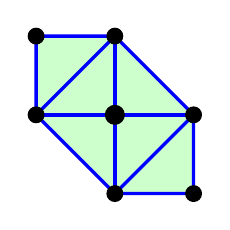
\begin{tikzpicture}

\draw [very thick, color=blue, fill=green, fill opacity=0.2]
(2,1) -- (3,1) -- (3,2) -- (2,3) -- (1,3) -- (1,2) -- cycle;

\draw [very thick, color=blue] (2,2) -- (3,2);
\draw [very thick, color=blue] (2,2) -- (2,3);
\draw [very thick, color=blue] (2,2) -- (2,1);
\draw [very thick, color=blue] (2,2) -- (1,2);
\draw [very thick, color=blue] (2,1) -- (3,2);
\draw [very thick, color=blue] (1,2) -- (2,3);


\draw [fill=black]  (2, 1) circle (0.1);
\draw [fill=black]  (3, 1) circle (0.1);
\draw [fill=black]  (3, 2) circle (0.1);
\draw [fill=black]  (2, 3) circle (0.1);
\draw [fill=black]  (1, 3) circle (0.1);
\draw [fill=black]  (1, 2) circle (0.1);
\draw [fill=black]  (2, 2) circle (0.12);
\end{tikzpicture}
\caption{The hexagon in another triangulation.}
\label{fig:trianghexagon}
\end{subfigure}
\begin{subfigure}{.4 \textwidth}

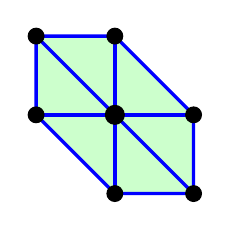
\begin{tikzpicture}

\draw [very thick, color=blue, fill=green, fill opacity=0.2]
(2,1) -- (3,1) -- (3,2) -- (2,3) -- (1,3) -- (1,2) -- cycle;

\draw [very thick, color=blue] (2,2) -- (3,2);
\draw [very thick, color=blue] (2,2) -- (2,3);
\draw [very thick, color=blue] (2,2) -- (2,1);
\draw [very thick, color=blue] (2,2) -- (1,2);
\draw [very thick, color=blue] (2,2) -- (3,1);
\draw [very thick, color=blue] (2,2) -- (1,3);


\draw [fill=black]  (2, 1) circle (0.1);
\draw [fill=black]  (3, 1) circle (0.1);
\draw [fill=black]  (3, 2) circle (0.1);
\draw [fill=black]  (2, 3) circle (0.1);
\draw [fill=black]  (1, 3) circle (0.1);
\draw [fill=black]  (1, 2) circle (0.1);
\draw [fill=black]  (2, 2) circle (0.12);
\end{tikzpicture}
\caption{The hexagon in the pulling triangulation.}
\end{subfigure}
\caption{Two triangulations of the hexagon.}
\label{fig:hexagon}
\end{figure}

In \figref{hexagon} are depicted two different triangulations of the hexagon. They correspond to different Gröbner bases of the ideal of $\dP6$. Choosing the left triangulation turns out to give smaller-dimensional $T^2$.

Below are some deformation computations done on the Stanley-Reisner scheme corresponding to the join of two hexagons in this triangulation.

\begin{lstlisting}
restart
R1 = QQ[x_1..x_6,y_0]
R2 = QQ[z_1..z_6,y_1]

loadPackage "SimplicialComplexes"
loadPackage "VersalDeformations"

S1 = simplicialComplex {x_1*x_2*x_3, x_1*y_0*x_3, x_3*x_4*y_0, x_6*x_1*y_0, x_6*x_4*y_0, x_6*x_5*x_4}
S2 = simplicialComplex {z_1*z_2*z_3, z_1*y_1*z_3, z_3*z_4*y_1, z_6*z_1*y_1, z_6*z_4*y_1, z_6*z_5*z_4}
I1 = ideal S1
I2 = ideal S2


R = QQ[first entries vars R1 | first entries vars R2]
I = sub(I1,R) + sub(I2,R)
\end{lstlisting}

We first create the rings with the necessary variables, then we define the simplicial complexes by their maximal faces. Finally we create the ideal of the join, which is just the sum of the individual ideals.

We can compute $T^2$:

\begin{lstlisting}
i11 :  CT^2(0, gens I);

              115       76
o11 : Matrix R    <--- R
\end{lstlisting}

It is $76$-dimensional, which is still quite big, but much smaller than if we had used the other triangulation.

We can compute $T^1$:

\begin{lstlisting}
i13 : T11 = CT^1(0, gens I);

              18       58
o13 : Matrix R   <--- R
\end{lstlisting}

This is the module of first-order deformations, which is $58$-dimensional.

Using the \texttt{VersalDeformations} package, we can lift the deformations to second order:
\begin{lstlisting}
(f1,r1,g1,c1) = versalDeformation(gens I, T11, CT^2(0, gens I),HighestOrder =>2, Verbose => 10);
\end{lstlisting}

Then \texttt{ideal sum g1} is the second order terms of the obstruction equations of the versal base space. The ideal is generated by $76$ elements, and by inspection we see that half of them uses only half of the deformation parameters. This makes it easier to compute a decomposition of it. We do it as follows:

\begin{lstlisting}
loadPackage "Binomials"
IG = ideal sum g1

IG1 = ideal ((IG_*)_{0..37})
IG2 = ideal ((IG_*)_{38..75})

T = QQ[t_1..t_27]
IGT1 = sub(IG1,T)
kList = BPD IGT1

T2 = QQ[t_28..t_58]
IGT2 = ideal mingens sub(IG,T2)
kList2 = BPD IGT2
\end{lstlisting}

This takes about a minute. We use the package \texttt{Binomials}, which decomposes binomial ideals fast. Finally, we put the decomposed parts in the same ring, and make a list of all the components:

\begin{lstlisting}
TT = QQ[t_1..t_58]
kListTT = apply(kList, I -> sub(I,TT))
kList2TT = apply(kList2, I -> sub(I,TT))

intersect(intersect kListTT, intersect(kList2TT)) ==  IGTT --- long time

comps = apply(toList ((set kListTT) ** (set kList2TT)), S -> ideal mingens (S#0 +S#1));
max apply(comps, dim) -- answer: 44
maxComp = select(comps, I -> dim I == 44)
\end{lstlisting}

We check which component has the maximal dimension, and it turns out that it has dimension $44$. We select that component in the last line. This ideal is generated by a subset of the deformation parameters.

We have been unable to lift this $44$-dimensional family, though. 

By selecting deformation parameters carefully, we can however find a family whose generic fiber is the ideal $J$ above (the sum of two del Pezzo's). This family is $8$-dimensional.

\begin{remark}
This is very promising, because of the following: we have found a smoothing of the singular Calabi-Yau inside $Y_0$, of which we computed the Euler characteristic to be $-72$. This fits well with the Batyrev-Borisov calculations above: if the Hodge numbers are $(8,44)$, we have potentially found an open subset of the moduli space of complex structures of this smoothing. The $8$-dimensional subfamily could correspond to the space of complex structures on the mirror.
\end{remark}

\section{Singularities}

\subsection{Of the toric hypersurface}

Again consider the join of two hexagons, joined with a single vertex. This is a 4-dimensional simplicial complex, which deforms to the toric variety with polytope with vertices $(v,0)$ and $(0,v)$, where $v$ are vertices of the hexagon. This is the same toric variety as in ``Second example'' above.

If \texttt{JJ} is the ideal of this toric variety, the following code will compute its singularities. 

\begin{lstlisting}
singlist = {}
for i from 1 to 6 do {
    sz = sub(JJ, z_i => 1);
    sx = sub(JJ, x_i => 1);
    singz = radical ideal mingens ideal singularLocus  minimalPresentation sz;
    singx = radical ideal mingens ideal singularLocus  minimalPresentation sx;
    singsx = (decompose singx);
    singsz = (decompose singz);
    sings = singsx | singsz;
    invz = sz.cache.minimalPresentationMap;
    invx = sx.cache.minimalPresentationMap;
    singlist = singlist | apply(singsx, I -> homogenize(preimage(invx, singx),x_i)) | apply(singsz, I -> homogenize(preimage(invz, singz),z_i));
    }
sings = intersect singlist
\end{lstlisting}

$X_P$ have $48$ curves as singularities. Hence a general hyperplane section will have $48$ isolated singularities.

\begin{remark}
Local calculations hint that these should be nodal singularities, but I don't immediately know how to see this.
\end{remark}

\section{Calabi-Yaus}

\subsection{Singular in a 5-dimensional toric}

Let $Y_0$ be the toric variety from \label{sec:toric5} embedded in $\P^{13}$ by (a subset of) the anticanonical system (use only the vertices and the origin). It is the join of two del Pezzo surfaces. The singular locus is the disjoint union of these del Pezzo surfaces. If we intersect $Y_0$ with two generic sections of the anticanonical bundle (in other words: two generic sections of $\OO_{Y_0}(1)$), we get a Calabi-Yau with isolated singularities.

In fact, local calculations on separate del Pezzos show that we don't need the hyperplanes to be generic. We'd like to have a Calabi-Yau on which a group act, so we want invariant hyperplanes. From Section \label{sec:delpezzoz2}, we know that $\Z_2 \X \Z_2$ act on each del Pezzo on $Y_0$. Hence we have a action of $\Z_2^5$ on $Y_0$, given by permuting each factor, and exchanging the factors.

\begin{remark}
We also have an action of $D_6 \times D_6 \times \Z_2$ on $Y_0$, but since we want the action to descend to the Calabi-Yau, we'd like invariant hyperplanes. However, this group is too big - there is only one invariant hyperplane with respect to this group (the hyperplane with all coefficients equal).
\end{remark}

There is a 3-dimensional vector space of invariant hyperplanes from $\OO_{Y_0}(1)$. We choose two of them:
\[
x_1+x_2+x_3+x_4+x_5+x_6+y_0+z_1+z_2+z_3+z_4+z_+5+z_6+y_1 = 0
\]
and
\[
x_1+x_2+2x_3+x_4+x_5+2x_6+y_0+z_1+z_2+2z_3+z_4+z_+5+2z_6+y_1 = 0.
\]
Local calculations show that this choice of hyperplanes give isolated singularities. They are all of the form $C(dP_6)$ and there are 12 of them. They come in two orbits under the group action: $4$ with a $\Z_2$ stabilizer, and $8$ with trivial stabilizer. The four with nontrivial stabilizer have coordinates
\begin{align*}
&\, (x_1:x_2:x_3:x_4:x_5:x_6:y_0:z_1:z_2:z_3:z_4:z_5:z_6:z_1)  \\
&= (0:0:0:1:-1:0:0:0:0:0:0:0:0:0), \\
&= (1:-1:0:0:0:0:0:0:0:0:0:0:0:0), \\
&= (0:0:0:0:0:0:0:0:0:0:1:-1:0:0), \\
&= (0:0:0:0:0:0:0:1:-1:0:0:0:0:0).
\end{align*}

The other $8$ have all nonzero coefficients with irrational coordinates. The exact coordinates can be computed symbolically in Mathematica for example.

The action have two fixed points that are not already singularities. The point $P_1$ with all cordinates equal to one is fixed. Also, the point $P_2$ with the first seven coordinates equal to $\lambda \neq 1,0$, and the last seven equal to $1$, is also fixed.

There are several points with nontrivial stabilizer [[find all of these]].

\section{Conceptual description}

Let $E$ be a rank $3$ vector space, and let $\PP^{17}=\PP(E \otimes E \oplus E \otimes E)$, thought of as the set of $3\times 3$ block matrices. Let $M$ be the set of block matrices having rank two. $M$ decomposes as $M=M' \cup M_1 \cup M_2$, where $M_i$ are the sets of block matrices where one of the blocks is zero, and the other has rank $2$. $M'$ is the subset of matrices where both blocks have rank exactly $1$. The dimensions are $9$, $4$, $4$.

The singular locus of (the closure of) $M'$ is the set of matrices $(0,B)$ and $(A,0)$, where $A,B$ have rank $1$.

If we intersect $M$ with a general $12$-plane (of codimension $6$), we therefore get a smooth Calabi-Yau $X$.

Let $S_3$ act on $E$ by permutations of a chosen basis. Then it act on $E \otimes E$ as well. The group $D_6 \simeq S_3 \times \Z_2$ act on the sum $E \otimes E \oplus E \otimes E$ by exchanging factors.

We choose a plane $H \simeq \PP^{11} \subset \PP^{17}$ such that $G$ act on it. There are several ways to do this. One way is to start with a generic $v_1 \otimes v_2 + v_3 \otimes v_4$ and let $G$ on this tensor. Since $G$ has order $12$, we get $12$ vectors (matrices) which span a $\PP^{11}$.

To get coordinates, let $x_i$ be coordinates on $\PP^{11}$. Let $A = \sum_{i=1}^{12} A_i x_i$. Then $X$ is defined by the $2\x 2$-minors of this block matrix.

\subsection{Elliptic fibration}

We have a map $\pi:M \bs \Sing(M) \to \PP^2 \times \PP^2$ defined as follows: generic elements of $M$ can be debscribed as being on the line between a pair of rank $1$ matrices $A$ and $B$. Write such an element as $A+\lambda B$. Rank $1$ matrices are parametrized by $\PP^2 \times \PP^2$, hence this family have dimension $4+1+4=9$, which fits nicely. The map is defined by sending $A+\lambda B$ to $A$.

We can restrict this map to $X=M \cap H$ to get a morphism $\pi:X \to \PP^2 \times \PP^2$. 


\subsection{Map to $(\PP^2)^{\times 4}$}

There is a map from $M' \backslash \Sing (M)$ to $(\PP^2)^4$ given by sending a pair of rank $1$ matrices $(A,B)$ to the tensor $v_1 \otimes v_2 \otimes v_3 \otimes v_4$, where $v_1 \otimes v_2 = A$ and $v_3 \otimes v_4=B$. The map has $\Aa^1 \bs pt$-fibers: the inverse image of a point is the line between $A$ and $B$: $\{ tA + s B\}_{(t:s) \in \Aa \bs 0}$. Let $\pi$ be this map.

Since $X$ doesnt intersect the singular locus of $M$, we get a map $\pi:X \to (\PP^2)^4$ by restriction. For generic choice of $\PP^{11}$, this map is injective. [[this should give us the Hodge numbers of X]]

\subsection{The invariant subfamily}

[[the invariant subfamily]]

\end{document}
